%%%%%%%%%%%%%%%%%%%%%%%%%%%%%%%%%%%%%%%%%
% University/School Laboratory Report
% LaTeX Template
% Version 3.1 (25/3/14)
%
% This template has been downloaded from:
% http://www.LaTeXTemplates.com
%
% Original author:
% Linux and Unix Users Group at Virginia Tech Wiki 
% (https://vtluug.org/wiki/Example_LaTeX_chem_lab_report)
%
% License:
% CC BY-NC-SA 3.0 (http://creativecommons.org/licenses/by-nc-sa/3.0/)
%
%%%%%%%%%%%%%%%%%%%%%%%%%%%%%%%%%%%%%%%%%

%----------------------------------------------------------------------------------------
%	PACKAGES AND DOCUMENT CONFIGURATIONS
%----------------------------------------------------------------------------------------

\documentclass{article}

\usepackage[version=3]{mhchem} % Package for chemical equation typesetting
\usepackage{siunitx} % Provides the \SI{}{} and \si{} command for typesetting SI units
\usepackage{graphicx} % Required for the inclusion of images
\usepackage{natbib} % Required to change bibliography style to APA
\usepackage{amsmath} % Required for some math elements 
\usepackage{hyperref}
\usepackage{subcaption}
\usepackage{float}
\usepackage{array}
\usepackage{amssymb}
\usepackage{calrsfs}
\usepackage{pgfplots}
\pgfplotsset{width=10cm,compat=1.9}
%\usepgfplotslibrary{external}
%\tikzexternalize


\setlength\parindent{0pt} % Removes all indentation from paragraphs

%\renewcommand{\labelenumi}{\alph{enumi}.} % Make numbering in the enumerate environment by letter rather than number (e.g. section 6)

%\usepackage{times} % Uncomment to use the Times New Roman font

%----------------------------------------------------------------------------------------
%	DOCUMENT INFORMATION
%----------------------------------------------------------------------------------------

\title{Homework \#4 \\Elliptic Curves \\[0.2em]\small{}CNS Course Sapienza} % Title and subtitle

\author{Riccardo \textsc{Prinzivalle}, 1904064} % Author name

\date{November 20, 2020} % Date for the report

\begin{document}

\maketitle % Insert the title, author and date

%----------------------------------------------------------------------------------------
%	SECTION 0
%----------------------------------------------------------------------------------------

\section{Homework Goal}

This homework contains a basic introduction on Elliptic Curves (EC), the general idea on the math basis, the Discrete Logarithm Problem with EC and the practical utilize of EC in cryptography.

%----------------------------------------------------------------------------------------
%	SECTION 1
%----------------------------------------------------------------------------------------

\section{Elliptic Curves Motivation}

Elliptic Curves are the main trend in asymmetric encryption today: why is their usage so spread? This question has a simple answer: it is sufficient to look at table \ref{tab:keyLen}, where there is a comparison of the key length needed to guarantee the same level of security. 
 
\renewcommand{\arraystretch}{2}

\begin{table}[H]
	\begin{center}
		\begin{tabular}{ |c || c | c | c | c | c | c | }
			\hline
			Algorithm Family & Cryptosystems & \multicolumn{4}{c |}{Security Level (bit)}\\
			& & 80 & 128 & 192 & 256\\ [0.5ex] 
			\hline\hline
			Integer Factorization & RSA & 1024 & 3072 & 7680 & 15360  \\ 
			
			Discrete Logarithm & DH, DSA, Elgamal & 1024 & 3072 & 7680 & 15360  \\ 
			
			Elliptic Curves & ECDH, ECDSA & 160 & 256 & 384 & 512  \\ 
			\hline
			Symmetric key & AES, 3DES &  80 & 128 & 192 & 256  \\ 
			\hline
		\end{tabular}
		\caption{Key length comparison in public key and symmetric key algorithm}
		\label{tab:keyLen}
	\end{center}
\end{table}

The bare minimum number of bits is defined by the symmetric key encryption scheme, we cannot have a smaller key with respect to the symmetric case and have the same level of security; then asymmetric schemes need, in general, a large number of bits to guarantee the same level of security, the fact is that elliptic curves cryptography needs less than $\cfrac{1}{10}$ of the bits needed for another asymmetric scheme supposed the same level of security, and this relationship become smaller as the level of security grows. Indeed, if one wants to use a public key cryptography scheme, elliptic curves are the suggested choice to guarantee security without using much computational effort.

%----------------------------------------------------------------------------------------
%	SECTION 2
%----------------------------------------------------------------------------------------

\section{Mathematical background}

The base idea besides elliptic curves lies on common calculus background: everyone knows the circumference equation, isn't it? It is $x^2 + y^2 = r^2$, but what if we add coefficients in front of the variables? We end up with an ellipse: $ax^2 + by^2 = r^2$, whose graph can be seen in Fig. \ref{fig:ellipse}. 

\begin{figure}[H]
	\centering
	\begin{subfigure}{.49\textwidth}
		\centering
		\begin{tikzpicture}
			\begin{axis}[
				xmin=-4,
				xmax=4,
				ymin=-6.6,
				ymax=7,
				xlabel={$x$},
				ylabel={$y$},
				scale only axis,
				axis lines=middle,
				domain=-4:4,      
				samples=1000,
				smooth,
				% use same unit vectors on the axis
				axis equal image=true,
				legend pos=south east,
				]
				\addplot [red] {sqrt(-0.2*x^2+2)};
				\addlegendentry{$y^2=-0.2x^2+2$};
				\addplot [red] {-sqrt(-0.2*x^2+2)};
			\end{axis}
		\end{tikzpicture}
		\caption{Ellipse}
		\label{fig:ellipse}
	\end{subfigure}
	\begin{subfigure}{.49\textwidth}
		\begin{tikzpicture}
			\begin{axis}[
				xmin=-4,
				xmax=4,
				ymin=-6.6,
				ymax=7,
				xlabel={$x$},
				ylabel={$y$},
				scale only axis,
				axis lines=middle,
				domain=-4:3,      
				samples=300,
				smooth,
				% use same unit vectors on the axis
				axis equal image=true,
				legend pos=south east,
				]
				\addplot [red] {sqrt(x^3-3*x+3)};
				\addlegendentry{$y^2=x^3-3x+3$};
				\addplot [red] {-sqrt(x^3-3*x+3)};
				\addplot [mark=none, domain=3:4, red, dashed] {sqrt(x^3-3*x+3)};
				\addplot [mark=none, domain=3:4, red, dashed] {-sqrt(x^3-3*x+3)};
			\end{axis}
		\end{tikzpicture}
		\centering
		\caption{Elliptic Curve}	
		\label{fig:EC}
	\end{subfigure}
	\caption{Graphical comparison of ellipse and elliptic curve}
	\label{fig:graph}
\end{figure}
 
 Well, an elliptic curve is something much similar: the general equation is $y^2 = x^3 + ax + b$, and an example of it can be seen in Fig. \ref{fig:EC}. We can easily see from the plot that this family of curves has symmetry with respect to $x$ axis. \newline
 In order to perform cryptography with elliptic curves, we need to reduce their usage to a special family of them: instead of defining them over the real domain $\mathbb{R}$, we use the integer group $\mathbb{Z}_{p}$ (which is a set of integer numbers with a group operator and is closed w.r.t. this operation), with $p > 3$. In addition, the elliptic curve equation is reduced in $mod p$, and the coefficient must satisfy the following equation to remove useless or too easy to break curves: $4a^3 + 27b^2 \ne{0}$. To fulfill the group operation, we need to add an imaginary point at infinity, $\mathcal{O}$. \newline
 Now that we have defined the elliptic curves of interest, we need to define a group over them, which is the basis of cryptography: in order to fulfill this task, we need a set of elements, which are the points belonging to the elliptic curves, and then we need a group operator to fulfill the group law. It is possible to have both a geometrical analytical interpretation of this operator; here we start with the geometrical one since it is easier to understand and more explicative.\newline
 The geometric interpretation starts by drawing the elliptic curve without modulo reduction and defined on $\mathbb{R}$, so we can easily visualize the curve in a 2D graph as those in Fig. \ref{fig:groupOp}. The group operation can be divided into 2 simpler case: the addition of two different point and the addition of the same point, called also doubling. 
 
 \begin{figure}[H]
 	\centering
 	\begin{subfigure}{.49\textwidth}
 		\centering
 		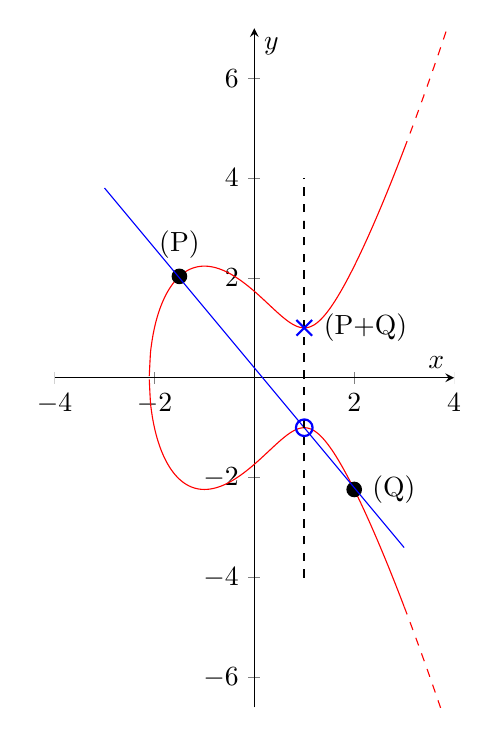
\begin{tikzpicture}[]
 			\begin{axis}[
 				xmin=-4,
 				xmax=4,
 				ymin=-6.6,
 				ymax=7,
 				xlabel={$x$},
 				ylabel={$y$},
 				scale only axis,
 				axis lines=middle,
 				domain=-4:3,      
 				samples=300,
 				smooth,
 				% use same unit vectors on the axis
 				axis equal image=true,
 				legend pos=south east,
 				]
 				\addplot [red] {sqrt(x^3-3*x+3)};
 				\addplot [red] {-sqrt(x^3-3*x+3)};
 				\addplot [mark=none, domain=3:4, red, dashed] {sqrt(x^3-3*x+3)};
 				\addplot [mark=none, domain=3:4, red, dashed] {-sqrt(x^3-3*x+3)};
 				\node[label={90:{(P)}},circle,fill,inner sep=2pt] at (axis cs:-1.5,{sqrt(4.125)}) {};
 				\node[label={0:{(Q)}},circle,fill,inner sep=2pt] at (axis cs:2,{-sqrt(5)}) {};
 				\addplot [blue, domain=-3:3] {-1.2*x+0.2};
 				\addplot [only marks,mark=o,color=blue,mark size=3, thick] coordinates { (1,{-sqrt(1)})};
 				\addplot[thick, samples=50, smooth, dashed] coordinates {(1,-4)(1,4)};
 				\addplot [only marks,mark=x,color=blue,mark size=4, thick] coordinates { (1,{sqrt(1)})};
 				\node[label={0:{(P+Q)}}] at (axis cs:1,{sqrt(1)}) {};
 			\end{axis}
 		\end{tikzpicture}
 		\caption{Point addition}
 		\label{fig:addition}
 	\end{subfigure}
 	\begin{subfigure}{.49\textwidth}
 		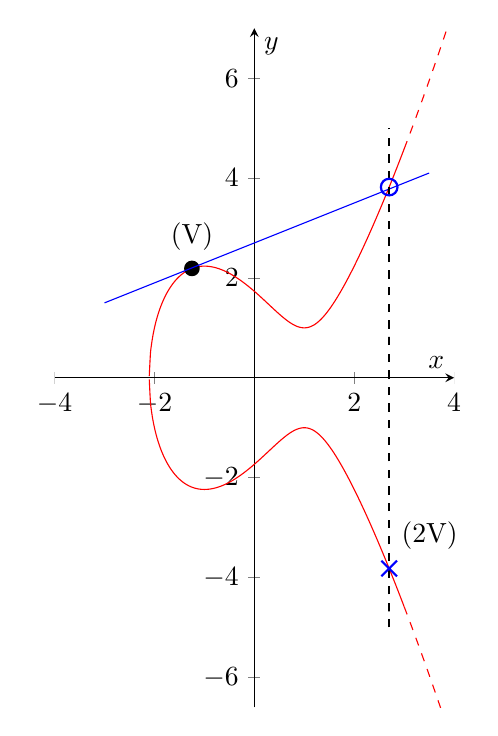
\begin{tikzpicture}
 			\begin{axis}[
 				xmin=-4,
 				xmax=4,
 				ymin=-6.6,
 				ymax=7,
 				xlabel={$x$},
 				ylabel={$y$},
 				scale only axis,
 				axis lines=middle,
 				domain=-4:3,      
 				samples=300,
 				smooth,
 				% use same unit vectors on the axis
 				axis equal image=true,
 				legend pos=south east,
 				]
 				\addplot [red] {sqrt(x^3-3*x+3)};
 				\addplot [red] {-sqrt(x^3-3*x+3)};
 				\addplot [mark=none, domain=3:4, red, dashed] {sqrt(x^3-3*x+3)};
 				\addplot [mark=none, domain=3:4, red, dashed] {-sqrt(x^3-3*x+3)};
 				\node[label={90:{(V)}},circle,fill,inner sep=2pt] at (axis cs:-1.25,{sqrt(4.796875)}) {};
 				%\node[label={90:{(P)}},circle,fill,inner sep=2pt] at (axis cs:-1.5,2.03) {};
 				%\node[label={0:{(Q)}},circle,fill,inner sep=2pt] at (axis cs:2,{-sqrt(5)}) {};
 				\addplot [blue, domain=-3:3.5] {0.4*x+2.7};
 				\addplot [only marks,mark=o,color=blue,mark size=3, thick] coordinates { (2.7,{sqrt(14.583)})};
 				\addplot[thick, samples=50, smooth, dashed] coordinates {(2.7,-5)(2.7,5)};
 				\addplot [only marks,mark=x,color=blue,mark size=4, thick] coordinates { (2.7,{-sqrt(14.583)})};
 				\node[label={75:{(2V)}}] at (axis cs:2.7,{-sqrt(14.583)}) {};
 			\end{axis}
 		\end{tikzpicture}
 		\centering
 		\caption{Point doubling}	
 		\label{fig:doubling}
 	\end{subfigure}
 	\caption{Graphical interpretation of group operator}
 	\label{fig:groupOp}
 \end{figure}

The first situation is represented in Fig. \ref{fig:addition}: we want to sum points P and Q, we draw the secant line passing through this two points, then, due to the particular form of the elliptic curve, we are able to find a new intersection between the EC and the secant other than the two point to be summed, this new point is highlighted by a circle in the figure, finally this point is mirrored w.r.t. the x axis and the resulting point is the sum between P and Q, and it is denoted by an \textit{x} in the plot.\newline
% TODO POINT DOUBLING 

%----------------------------------------------------------------------------------------
%	SECTION 3
%----------------------------------------------------------------------------------------

\section{Discrete Logarithm Problem with Elliptic Curves}


\begin{figure}[H]
\centering
\begin{subfigure}{.54\textwidth}
  \centering
  %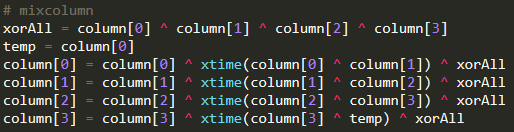
\includegraphics[width=1\linewidth]{images/mixcolumn.png}
  \caption{Core}
  \label{fig:core}
\end{subfigure}
\begin{subfigure}{.35\textwidth}
  \centering
  %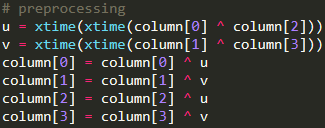
\includegraphics[width=1\linewidth]{images/preprocessing.png}
  \caption{Preprocessing}
  \label{fig:preprocessing}
\end{subfigure}
\caption{Mix columns base functions}
\label{fig:MixColumns}
\end{figure}
 
%----------------------------------------------------------------------------------------
%	SECTION 4
%----------------------------------------------------------------------------------------

\section{Use of Elliptic Curves in Cryptography}


%----------------------------------------------------------------------------------------
%	SECTION 5
%----------------------------------------------------------------------------------------

\section{Conclusion}



%----------------------------------------------------------------------------------------
%	BIBLIOGRAPHY
%----------------------------------------------------------------------------------------

\bibliographystyle{abbrv}

%\bibliography{sample}

%----------------------------------------------------------------------------------------


\end{document}